% HW2 paper (ACL format). Build: pdflatex -> bibtex -> pdflatex x2 (VS Code: LaTeX Workshop, see .vscode/).
% main.tex        -> named version, \usepackage[preprint]{acl}  -> HW2_<TeamID>_report.pdf
% main_review.tex -> anonymized version, \usepackage[review]{acl}, Team ID only (LLM TA Judge draft)
\providecommand{\anonymous}{0}
\documentclass[11pt]{article}

\ifnum\anonymous=1
  \usepackage[review]{acl}
  % Keep review mode (line numbers) but print the Team ID instead of "Anonymous ACL submission",
  % as the assignment asks; acl.sty itself stays unmodified.
  \makeatletter\acl@anonymizefalse\makeatother
\else
  \usepackage[preprint]{acl}
\fi

\usepackage{times}
\usepackage{latexsym}
\usepackage[T1]{fontenc}
\usepackage[utf8]{inputenc}
\usepackage{microtype}
\usepackage{inconsolata}
\usepackage{graphicx}
\usepackage{amsmath}
\usepackage{amssymb}
\usepackage{booktabs}
\usepackage{enumitem}
\setlist{nosep, leftmargin=*}
\usepackage{tikz}
\usetikzlibrary{positioning,arrows.meta}

% Figures are read straight from the experiment outputs.
\graphicspath{{../results/}}

% TODO: fill in the team ID and every member's name and student ID.
\newcommand{\teamid}{Team TODO}
\newcommand{\repourl}{\url{https://github.com/calculusfkyou/nycu-data-mining-assignment-2-115-1}}

\title{TODO: Paper Title}

\ifnum\anonymous=1
  \author{\teamid}
\else
  \author{\teamid \\
    TODO Member A (student ID) \quad
    TODO Member B (student ID) \quad
    TODO Member C (student ID) \\
    {\normalfont\small \repourl}}
\fi

\begin{document}
\maketitle

% !TEX root = ../main.tex
% Numbers from results/stage6_main/summary.csv, results/stage8_analysis/{significance,peak_in_mask}.csv.
\begin{abstract}
Quality-control inspectors need a camera-based detector that flags defective products for rejection or
manual re-inspection, learned from normal images because defects are rare and varied.
We study this on VisA, 10,821 industrial images of 12 objects with defects covering a median 0.20\% of
the image, and compare three tiers on one leakage-free split with per-object thresholds chosen on a
labelled validation set: a template difference, PaDiM (a Gaussian per location on pretrained features,
our primary method) and PatchCore.
PaDiM reaches 0.801\,$\pm$\,0.007 PR-AUC, PatchCore 0.885\,$\pm$\,0.002, a significant gap
($+0.084$, bootstrap 95\% CI $[0.065, 0.102]$).
At a 1\% defect rate, however, only 3.7\% and 14.8\% of their alerts are real defects.
Ablations show that PaDiM depends on its location-wise covariance, and error analysis traces its
failures to position: its anomaly map peaks inside the defect for 25\% of anomalies, against 70\% for
PatchCore.
\end{abstract}

% !TEX root = ../main.tex
\section{Introduction}
\label{sec:intro}

TODO

% !TEX root = ../main.tex
% §2 Related Work. Every number in Table~\ref{tab:related} was checked against the cited paper:
% SPADE / Rippel / PaDiM on MVTec AD from Table 2 of Defard et al.; PatchCore on MVTec AD from its abstract;
% VisA rows from Tables 2 and 6 of Zou et al.; "Ours" from results/stage6_main/summary.csv (12 classes).
\section{Related Work}
\label{sec:related}

\paragraph{Benchmarks and methods.}
Our task is in the image data category, where industrial inspection is usually studied on MVTec AD
\citep{bergmann2019mvtec}, where image-level AUROC is close to saturated (Table~\ref{tab:related}).
VisA \citep{zou2022spot} adds complex structures and freely placed instances, and the same PatchCore drops
there from 99.8 to 92.4 AUROC, so it still separates methods.
Among the families reviewed by \citet{ruff2021unifying}, the strongest normal-only detectors on such data
pair ImageNet-pretrained features with a simple model: a global Gaussian \citep{rippel2021modeling}, a
Gaussian per location (PaDiM, \citealp{defard2021padim}), or $k$NN to normal patches (SPADE,
\citealp{cohen2020spade}; PatchCore, \citealp{roth2022towards}).

\begin{table*}[t]
  \centering
  \small
  \setlength{\tabcolsep}{5pt}
  \begin{tabular}{@{}lllccc@{}}
    \toprule
    Work & Data & Method (family), backbone & Paradigm & AUROC & AU-PR \\
    \midrule
    \citet{cohen2020spade}     & MVTec AD & SPADE (patch $k$NN), WRN50 & normal only & 85.5$^\dagger$ & -- \\
    \citet{rippel2021modeling} & MVTec AD & global Gaussian, EfficientNet-B4 & normal only & 95.8 & -- \\
    \citet{defard2021padim}    & MVTec AD & PaDiM (patch Gaussian), WRN50 & normal only & 95.3 & -- \\
    \citet{roth2022towards}    & MVTec AD & PatchCore (patch $k$NN) & normal only & up to 99.6 & -- \\
    \citet{zou2022spot}        & VisA & PaDiM (patch Gaussian), ResNet-50 & normal only & 87.8 & 88.2 \\
    \citet{zou2022spot}        & VisA & PatchCore (patch $k$NN), WRN50 & normal only & 92.4 & 93.3 \\
    \midrule
    Ours, Tier 2 & VisA$^\ast$ & PaDiM (patch Gaussian), WRN50 & normal + val.\ $\tau$ & 82.8\,$\pm$\,0.8 & 80.1\,$\pm$\,0.7 \\
    Ours, Tier 3 & VisA$^\ast$ & PatchCore (patch $k$NN), WRN50 & normal + val.\ $\tau$ & 90.2\,$\pm$\,0.2 & 88.5\,$\pm$\,0.2 \\
    \bottomrule
  \end{tabular}
  \caption{Image-level results (\%) of prior work and ours. ``Normal + val.\ $\tau$'': labelled val
    anomalies only choose thresholds and hyperparameters. $^\dagger$As reported by
    \citet{defard2021padim}. $^\ast$Our split (\S\ref{sec:data}): context, not a direct comparison;
    mean\,$\pm$\,std over 3 seeds, 12 objects.}
  \label{tab:related}
\end{table*}

\paragraph{Choice of tiers and positioning.}
The tiers differ in what they assume about normal images.
Tier~1 (template difference) assumes pixel alignment and is a lower bound.
Tier~2 (PaDiM) assumes one Gaussian per feature location; it is cheap, interpretable per location and
has few hyperparameters, so it is our primary method.
Tier~3 (PatchCore) drops the alignment assumption at the cost of a memory bank.
Unlike prior VisA work, which reports threshold-free scores on an official test set that is 55\%
anomalous, we fix thresholds on a labelled validation split and report operating points at a 1\% and
5\% deployment prevalence.

% !TEX root = ../main.tex
% §3 Task Definition & Data. Numbers from results/stage4_eda/{eda_summary,eda_split_counts,eda_imbalance,
% eda_crop_loss}.csv; Tier 2 feature size from results/stage6_main/search_log.txt (chosen config).
\section{Task Definition \& Data}
\label{sec:data}

\paragraph{Anomaly definition and unit of detection.}
This is an image anomaly detection task: industrial inspection photographs, where the challenge is
spatial texture, background clutter and very small defects.
The unit of detection is one image of one product.
An image is \emph{normal} if the object meets specification, and \emph{anomalous} if it shows a surface
defect (scratch, burn, colour spot, crack, bubble) or a structural defect (bent, misplaced or missing
part).
Figure~\ref{fig:samples} shows one normal and one anomalous image for four objects.
The defects are small: the median ground-truth mask covers 0.20\% of the image (10th / 90th
percentile: 0.03\% / 1.67\%).

\begin{figure*}[t]
  \centering
  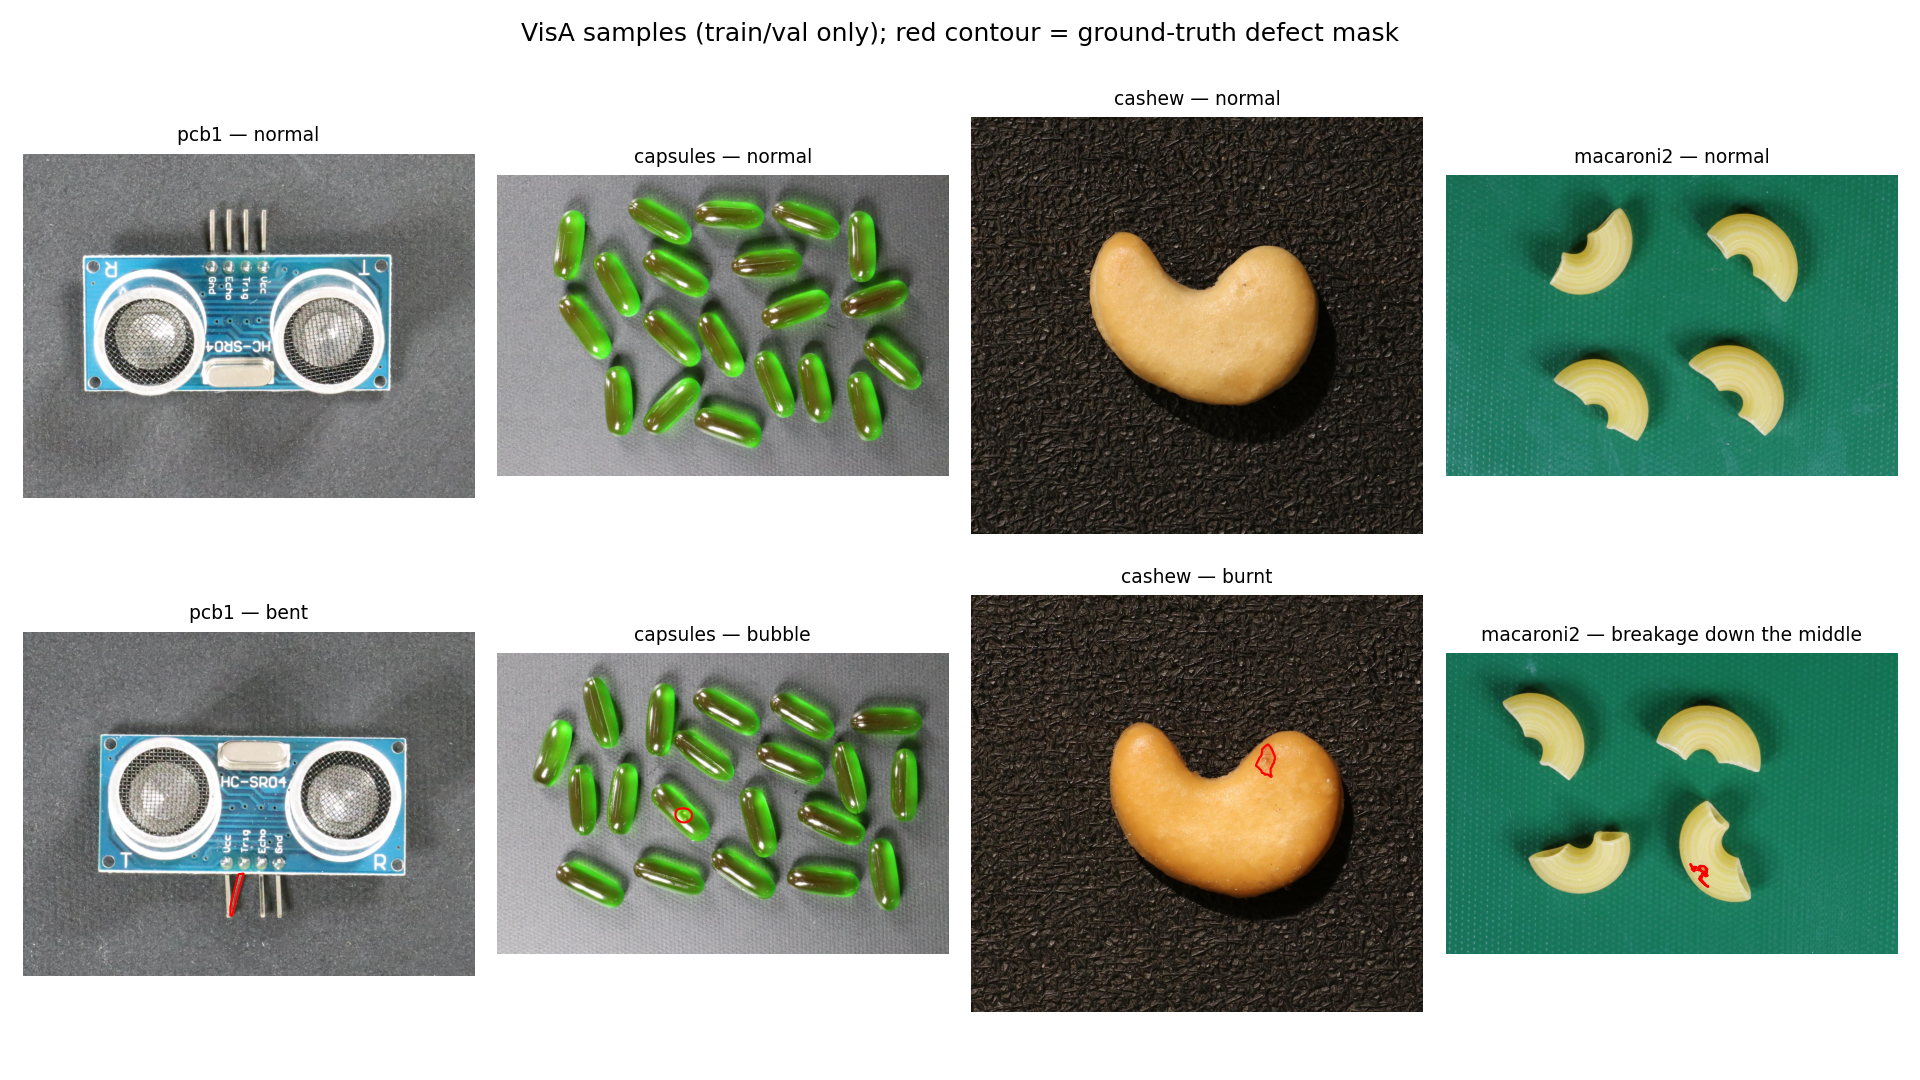
\includegraphics[width=0.8\textwidth]{stage4_eda/fig_samples.png}
  \caption{Normal (top) and anomalous (bottom) VisA images for four of the 12 objects, taken from train and
    validation only. Red contours mark the ground-truth defect masks.}
  \label{fig:samples}
\end{figure*}

\paragraph{Dataset.}
We use VisA \citep{zou2022spot}, released under CC BY 4.0 at
\url{https://github.com/amazon-science/spot-diff}.
It contains $N = 10{,}821$ images, of which 9,621 are normal and 1,200 anomalous.
They cover 12 objects in three groups: complex structure (pcb1--4), multiple instances (candle, capsules,
macaroni1--2) and single instance (cashew, chewing gum, fryum, pipe fryum), with 34 defect types in total.
Raw images are 1,274--1,562\,px wide and 960--1,176\,px high.
Every tier receives a $224 \times 224 \times 3$ input ($D = 150{,}528$).
Tiers~2 and~3 work on pretrained patch features instead of pixels: 3,584 channels per location for
Tier~2 (reduced to 200, \S\ref{sec:method}) and 1,536 for Tier~3.
Table~\ref{tab:data} summarises the data.

\paragraph{Labels and paradigm.}
Image-level labels and pixel masks are provided by the dataset authors; we use the masks only for
analysis, never for training.
Subtle defects may carry label noise, which we cannot quantify.
For capsules every anomaly carries the same defect label (bubble), so the per-type stratification
below reduces to random sampling for that object.
The setting is semi-supervised: every model is fitted on normal images only, and a small set of labelled
anomalies is used only to choose thresholds and hyperparameters.

\paragraph{Split.}
Starting from the official one-class split, we fix one split (seed~0) and share it across all tiers
(Table~\ref{tab:data}).
For each object, 89\% of the official training normals form \emph{train}.
The other 11\% plus 20 anomalies form \emph{val}.
Another 20 anomalies form a \emph{contamination pool}, used only in the training-contamination
ablation.
The official test normals plus the remaining 60 anomalies form \emph{test}.
Anomalies are stratified by defect type, and no image appears in two splits.

\begin{table}[t]
  \centering
  \small
  \begin{tabular}{@{}lrrr@{}}
    \toprule
    Subset & Normal & Anomaly & Anomaly \% \\
    \midrule
    Full dataset       & 9,621 & 1,200 & 11.1 \\
    Train              & 7,705 &     0 &  0.0 \\
    Val                &   954 &   240 & 20.1 \\
    Contamination pool &     0 &   240 & -- \\
    Test               &   962 &   720 & 42.8 \\
    \midrule
    \multicolumn{4}{@{}l}{Objects 12; defect types 34; median defect area 0.20\%} \\
    \multicolumn{4}{@{}l}{Raw size $\approx$1,400\,$\times$\,1,070\,px; input $224 \times 224 \times 3$} \\
    \bottomrule
  \end{tabular}
  \caption{VisA summary and our split (all 12 objects). Train, val and test use 20 / 20 / 60
    anomalies per object; ``raw size'' is the median width $\times$ height.}
  \label{tab:data}
\end{table}

\paragraph{Preprocessing.}
Images are resized directly to $224 \times 224$ and normalised with ImageNet statistics.
We do not use the common resize-256 plus centre-crop-224.
On val masks that crop would remove 4.1\% of defect pixels on average, 10.9\% for capsules and 22.9\% for
macaroni2, where 12.5\% of the defects would be cut out entirely.

\paragraph{Class imbalance.}
The anomaly : normal ratio is 1 : 8.02 over the full dataset (11.1\% anomalies), 1 : 3.98 in val and
1 : 1.34 in test (42.8\%).
Both are far above a realistic production prevalence.
A predict-all-normal rule reaches 57.2\% test accuracy, and would reach 99.0\% at a 1\% prevalence while
catching no defect, so we never report accuracy.
A classifier trained with plain cross-entropy on such data would drift towards the same rule.
We avoid that failure in three ways.
First, all models are fitted on normal images only, so the rare class never enters a loss.
Second, the primary metric is PR-AUC, which, unlike ROC-AUC, depends on the anomaly rate
\citep{davis2006relationship,saito2015precision}.
Third, we convert each operating point to the precision expected at a deployment prevalence $\pi$:
\begin{equation}
  \mathrm{prec}_\pi = \frac{\pi \cdot \mathrm{TPR}}{\pi \cdot \mathrm{TPR} + (1-\pi) \cdot \mathrm{FPR}},
  \label{eq:prec-pi}
\end{equation}
with $\pi \in \{1\%, 5\%\}$.

% !TEX root = ../main.tex
\section{Exploratory Feature Analysis}
\label{sec:eda}

TODO

% !TEX root = ../main.tex
\section{Method}
\label{sec:method}

TODO

% !TEX root = ../main.tex
% §6 Experimental Setup. Search: results/stage6_main/search_log.txt (config ids follow run.py GRID order);
% environment.csv and latency.csv, peak memory from main_log.txt. The main run (stages 5-8) used the
% environment in environment.csv (see README); requirements.txt pins the stage 1-4 environment.
\section{Experimental Setup}
\label{sec:setup}

\paragraph{Split and leakage prevention.}
All tiers use the single split of \S\ref{sec:data} (fixed indices, seed~0): 7,705 / 1,194 / 1,682
images for train / val / test.
Models are fitted on train normals only.
Preprocessing uses fixed ImageNet statistics, so nothing is fitted on val or test.
Val anomalies are used only to choose $\tau$ and the hyperparameters below, never to fit weights.
For every object, all models are fitted and all thresholds fixed before the test features are loaded,
and test is evaluated once.
The only earlier contact with test was a pipeline smoke test on one object (candle, seed~0, default
settings) before the search; nothing was chosen from it.

\paragraph{Hyperparameters.}
The search uses val only (seed~0).
For each tier it fits every point of the grid in Table~\ref{tab:hparams} and keeps the setting with the
highest mean val PR-AUC over the 12 objects.
The chosen Tier~2 setting lies at the edge of its grid; we kept the grid as defined in advance.

\begin{table}[t]
  \centering
  \small
  \setlength{\tabcolsep}{4pt}
  \begin{tabular}{@{}llll@{}}
    \toprule
    Tier & Hyperparameter & Range & Selected \\
    \midrule
    T2 & channels $d$ & 50, 100, 200 & 200 \\
    T2 & layers & \{2,3\}, \{2,3,4\} & \{2,3,4\} \\
    T2 & ridge $\epsilon$ & fixed & 0.01 \\
    \midrule
    T3 & coreset ratio & 1\%, 10\% & 1\% \\
    T3 & layers & \{2,3\}, \{2,3,4\} & \{2,3\} \\
    T3 & neighbourhood / proj. & fixed & $3 \times 3$ / 128-d \\
    \bottomrule
  \end{tabular}
  \caption{Hyperparameter search on val (seed~0, full grid per tier). Mean val PR-AUC of the selected
    setting: 0.664 (T2) and 0.811 (T3).}
  \label{tab:hparams}
\end{table}

\paragraph{Metrics.}
PR-AUC is the primary metric because, unlike ROC-AUC, it reflects how many alerts are real defects under
class imbalance \citep{davis2006relationship,saito2015precision}.
We also report ROC-AUC for comparison with the literature.
At the chosen $\tau$ we report F1, F2 and the false-positive rate, which is the share of good products
sent to re-inspection.
We also report $\mathrm{prec}_\pi$ (Eq.~\ref{eq:prec-pi}) at $\pi = 1\%$ and $5\%$, the share of alerts
that would be real defects in production.
Every number is the mean $\pm$ std over seeds 0, 1 and 2 of the 12-object average.
The seed controls the Tier~2 channel subset and the Tier~3 coreset start and projection; Tier~1 is
deterministic.

\paragraph{Implementation and hardware.}
PyTorch 2.15.0 with CUDA 13.2, torchvision 0.29.2 and scikit-learn, on an NVIDIA RTX 4060 Ti (8\,GB).
Latency is the median over 50 val images of pcb1, on GPU with batch size~1 after 10 warm-up images,
including feature extraction.
Training time covers model fitting only, not loading the cached features.
The main run peaked at 2.24\,GB of GPU memory and 6.6\,GB of RAM.

% !TEX root = ../main.tex
% §7 Results. Main table: results/stage6_main/summary.csv and latency.csv; significance:
% results/stage8_analysis/significance.csv (src/analyze.py, N_BOOT = 1000); ablations:
% results/stage7_ablation/ablation_summary.csv.
\section{Results}
\label{sec:results}

\begin{table*}[t]
  \centering
  \footnotesize
  \setlength{\tabcolsep}{3pt}
  \begin{tabular}{@{}lcccccccc@{}}
    \toprule
    Method & PR-AUC & ROC-AUC & F1 & F2 & FPR$\downarrow$ & prec$_{1\%}$ & ms/img$\downarrow$ & fit s$\downarrow$ \\
    \midrule
    T0 all normal & 0.442 & 0.500 & 0 & 0 & 0 & -- & -- & -- \\
    T1 template & 0.702 & 0.762 & 0.693 & 0.767 & 0.465 & 0.018 & \textbf{0.12}$^\ast$ & \textbf{0.1} \\
    T2 PaDiM & 0.801\,$\pm$\,0.007 & 0.828\,$\pm$\,0.008 & 0.733\,$\pm$\,0.007 & 0.779\,$\pm$\,0.006
      & 0.332\,$\pm$\,0.012 & 0.024\,$\pm$\,0.001 & 7.38 & 2.8 \\
    T3 PatchCore & \textbf{0.885}\,$\pm$\,0.002 & \textbf{0.902}\,$\pm$\,0.002 & \textbf{0.806}\,$\pm$\,0.009
      & \textbf{0.808}\,$\pm$\,0.008 & \textbf{0.174}\,$\pm$\,0.021 & \textbf{0.046}\,$\pm$\,0.005 & 11.72 & 114 \\
    \bottomrule
  \end{tabular}
  \caption{Test results averaged over the 12 objects, mean\,$\pm$\,std over 3 seeds (T0 and T1 are
    deterministic); best per column in bold, T0 excluded. prec$_{1\%}$: Eq.~\ref{eq:prec-pi} at
    $\pi = 1\%$ from the object-averaged TPR and FPR of each seed (per object it is unreliable: with
    50--101 test normals, FPR is often 0). ms / img: median GPU latency incl.\ feature extraction ($^\ast$T1 on CPU, no backbone);
    fit: total over 12 objects. Without cashew, pcb1 and pcb2, PR-AUC is 0.655 / 0.785 / 0.874 for
    T1 / T2 / T3.}
  \label{tab:main}
\end{table*}

\paragraph{Main results.}
Tier~3 beats Tier~2 (Table~\ref{tab:main}) on 11 of 12 objects by $+0.084$ PR-AUC, a significant gap:
paired bootstrap 95\% CI $[0.065, 0.102]$ (test images resampled within object and label, 1,000
rounds), Wilcoxon $p = 0.003$ over objects, paired $t$-test $p = 0.003$ over seeds.
Without the three flagged objects it is $+0.089$ $[0.067, 0.109]$, $p = 0.012$.
Tier~2 beats Tier~1 by $+0.099$ but only on 9 of 12 objects ($p = 0.077$), a trend rather than a
significant gain.
Our Tier~3 ROC-AUC (90.2) is 2.2 points below the 92.4 reported on the official split
\citep{zou2022spot}, plausible for a re-implementation on a different test set.

\paragraph{Why Tier 2 loses.}
Tier~2 expects each part of the object at a fixed location, whereas Tier~3 matches patches from any
position; this robustness costs 41$\times$ the training time (114\,s vs.\ 2.8\,s, paid once) and
4.3\,ms more per image.
F2 hides the gap because the test set is 43\% anomalous (Tier~1 reaches F2 0.767 at FPR 0.465); at a
1\% prevalence only 2.4\% of Tier~2 and 4.6\% of Tier~3 alerts would be real defects.

\begin{table}[t]
  \centering
  \small
  \setlength{\tabcolsep}{3pt}
  \begin{tabular}{@{}llcc@{}}
    \toprule
    Factor & Setting & PR-AUC & $\Delta$ \\
    \midrule
    -- & full Tier 2 & 0.801\,$\pm$\,0.007 & -- \\
    \midrule
    Scoring & Euclidean 1-NN & 0.734\,$\pm$\,0.003 & $-0.067^\ast$ \\
            & cosine 1-NN    & 0.686\,$\pm$\,0.021 & $-0.115^\ast$ \\
    Contam. & 1\% of train & 0.797\,$\pm$\,0.007 & $-0.004$ \\
                  & 2\% of train & 0.794\,$\pm$\,0.008 & $-0.007$ \\
    Aggregation & top-1\% mean          & 0.799\,$\pm$\,0.006 & $-0.002$ \\
                & smoothed max &0.796\,$\pm$\,0.007 & $-0.004$ \\
    Features & global pooled & 0.771\,$\pm$\,0.006 & $-0.029^\ast$ \\
    \bottomrule
  \end{tabular}
  \caption{Tier~2 ablations, one factor at a time (12 objects, 3 seeds). $^\ast$: $|\Delta|$ exceeds
    the seed std of both settings. Full Tier~2: Mahalanobis, 0\% contamination, max, patch-level; smoothed max uses
    $\sigma = 4$.}
  \label{tab:ablation}
\end{table}

\paragraph{Controlled ablations.}
In Table~\ref{tab:ablation} the location-wise covariance matters most: a nearest-neighbour distance at
the same location costs 0.07--0.12 PR-AUC.
Pooling the map into one global vector costs 0.029 (0.038 on nine objects), in line with H2 (\S
ef{sec:analysis}).
The threshold rule leaves PR-AUC unchanged but moves the operating point beyond seed std: from best-F2
(recall / FPR / prec$_{1\%}$ = 0.82 / 0.33 / 0.024) to best-F1 (0.64 / 0.18 / 0.035), a top-10\% review
budget (0.35 / 0.04 / 0.082) or the 99th percentile of val normals (0.29 / 0.02 / 0.138).
Two results are negative.
Adding 1--2\% anomalies to train (4--16 images per object; our pool of 20 per object rules out 5\% and
10\%) changes PR-AUC by less than the seed std, likely because a median defect covers only 0.20\% of
the image, so far fewer than 2\% of \emph{locations} are contaminated.
Aggregation and the smoothing of \citet{defard2021padim} have no effect either, so H3 is not supported.

% !TEX root = ../main.tex
\section{Analysis}
\label{sec:analysis}

TODO

% !TEX root = ../main.tex
\section{Conclusion \& Limitations}
\label{sec:conclusion}

TODO

% !TEX root = ../main.tex
% Counts toward the 6-page limit; must come before the references.
\section*{Contributions of Each Member}
\begin{itemize}
  \item TODO Member A (student ID): ...
  \item TODO Member B (student ID): ...
  \item TODO Member C (student ID): ...
\end{itemize}

\paragraph{AI usage statement.}
TODO: tools and versions, the steps they were used for, and which decisions the team made and verified.


\bibliography{references}

\end{document}
